
\documentclass{article}

\usepackage[english]{babel} % babel specifies the language
\usepackage[utf8]{inputenc} % this one is...confusing
\usepackage{graphicx} % graphicx handles graphics
\usepackage[margin=1in]{geometry}
\usepackage{bbm}
\usepackage{amsmath,amssymb}
\usepackage{wasysym}
\usepackage{listings}
\usepackage{graphicx}
\usepackage[font={footnotesize}]{caption}
\usepackage{subcaption}
\usepackage{multicol}
\usepackage{wrapfig}

\lstset{
  basicstyle=\small\ttfamily,        % the size of the fonts that are used for the code
  breakatwhitespace=false,         % sets if automatic breaks should only happen at whitespace
  breaklines=true,                 % sets automatic line breaking
  captionpos=b,                    % sets the caption-position to bottom
  extendedchars=true,              % lets you use non-ASCII characters; for 8-bits encodings only, does not work with UTF-8
  frame=single,                    % adds a frame around the code
  language=Java,                 % the language of the code
  keywordstyle=\bf,
  showspaces=false,                % show spaces everywhere adding particular underscores; it overrides 'showstringspaces'
  showstringspaces=false,          % underline spaces within strings only
  showtabs=false,                  % show tabs within strings adding particular underscores
  tabsize=2                       % sets default tabsize to 2 spaces
}

\DeclareMathOperator{\E}{\mathbb{E}}

\title{Adaboost for forest cover - Statistical methods for machine learning}
\author{Bertolotti Francesco}
\date{Jun 2019} % \today will print the compile date

\begin{document}
\maketitle

\section{Algorithm Description}
\subsection{Adaboost}

The general idea is to get a predictor from a weighted sum of other predictors, using appropriate weights.\\\\
Let $D$ be the joint distribution of $X\times Y = D$, where $X \in \mathcal{X}$ and $Y \in \mathcal{Y}$ and 
$\mathcal{Y} =\{-1,+1\}$.\\
Let $S$ be the training set, such that $S=\{(x_t,y_t)\}_{t=1}^{m}$.
where each $(x_t, y_t)$ is drawn from $D$.\\
Let $l$ be the $0/1$ loss functions, such that $l(y,\hat{y}) = \mathbbm{1}{\{y \neq \hat{y}\}}$. \\
Let $l_S:H\rightarrow[0,1]$ be the training loss, $l_S(h) = \frac{1}{m}\sum_{t=1}^{m} l(h(x_t),y_t)$,
for $h\in H$.\\
Let $l_D:H\rightarrow[0,1]$ be the statistical loss, $l_D(h) = \underset{X,Y \sim D}{\E} [l(h(X),Y)]$.\\
Let $h_1, h_2, \dots, h_T$ be predictors, such that $\forall i=1,2,\dots,T : h_t:\mathcal{X}\rightarrow\mathcal{Y}$.\\

Adaboost will output the following predictor $f$:
$$f(x) = sgn(\sum_{i=1}^{T}w_i h_i(x))$$.

Adaboost finds the weights $w_i$ such that the training error is low.\\

\begin{align*}
l_S(f) = \frac{1}{m}\sum_{t=1}^{m}l(f(x_t),y_t) 
       = \frac{1}{m}\sum_{t=1}^{m}\mathbbm{1}\{f(x_t) \neq y_t \}
       = \frac{1}{m}\sum_{t=1}^{m}\mathbbm{1}\{f(x_t) y_t \leq 0 \} =\\
       \leq \frac{1}{m}\sum_{t=1}^{m}e^{-f(x_t)y_t}
       = \frac{1}{m}\sum_{t=1}^{m}e^{-\sum_{i=1}^{T}w_i h_i(x_t) y_t}
       = \frac{1}{m} \sum_{t=1}^{m} \prod_{i=1}^{T} e^{-w_i h_i(x_t) y_t} =\\
       = \E_{t\sim \mathbb{P}_1} [\prod_{i=1}^{T} e^{-w_i h_i(x_t) y_t}] 
       \stackrel{(*)}{=} \prod_{i=1}^{T} \E_{t\sim \mathbb{P}_i} [ e^{-w_i h_i(x_t) y_t} ] =\\
       = \prod_{i=1}^{T} e^{-w_i} \mathbb{P}_i(h_i(x_t) y_t = +1) + e^{w_i} \mathbb{P}_{i}(h_i(x_t) y_t = -1) 
       = \prod_{i=1}^{T} e^{-w_i} (1-\epsilon_i) + e^{w_i} \epsilon_i.\\
\end{align*}

now we find $w_i$ such that: $w_i = \underset{w}{argmin} \{ e^{-w}(1-\epsilon_i) + e^{w} \epsilon_i \}$.

\begin{align*}
\frac{d}{dw}e^{-w}(1-\epsilon_i) + e^{w} \epsilon_i = 0 \implies
e^{w}\epsilon_i = e^{-w}(1-\epsilon_i).
\end{align*}



\[
\begin{cases} 
\epsilon_i = 1 \implies e^{w} = 0 \text{ \lightning}.\\
\epsilon_i = 0 \implies e^{-w} = 0 \text{ \lightning}.\\
0 < \epsilon_i < 1  \implies  w ln(e) + ln(\epsilon_i) = -w ln(e) + ln(1-\epsilon_i).
\end{cases}
\]


\begin{align*}
w ln(e) + ln(\epsilon_i) = -w ln(e) + ln(1-\epsilon_i)\implies
w =  \frac{1}{2}ln(\frac{1-\epsilon_i}{\epsilon_i}).
\end{align*}

continuing from $(4)$... 

\begin{align*}
\prod_{i=1}^{T} e^{\frac{1}{2}ln(\frac{\epsilon_i}{1-\epsilon_i})} (1-\epsilon_i) + e^{\frac{1}{2}ln(\frac{1-\epsilon_i}{\epsilon_i})} \epsilon_i.
= \prod_{i=1}^{T} 2\sqrt{(1-\epsilon_i)\epsilon_i}.
\end{align*}

Now, call $\gamma_i = \frac{1}{2}-\epsilon_i$.

\begin{align*}
\prod_{i=1}^{T} 2\sqrt{(1-\epsilon_i)\epsilon_i} =
\prod_{i=1}^{T} \sqrt{(1-4\gamma_i^2)} = 
\prod_{i=1}^{T} e^{-2\gamma_i^{2}} = 
e^{-\sum_{i=1}^{T} 2\gamma_i^{2}} \leq
e^{-2T\gamma^2}.
\end{align*}

where $\gamma = \underset{i}{min} \{ \gamma_i \}$. \\

Which means that the training error decreases exponentially in the number of $T$.
Now note that $\epsilon_i$ was $\mathbb{P}_i(h_i(x_t) y_t = -1)$, 
that is, the probability of $h_i$ making a mistake on the training set $S$ 
where each sample is weighted by $\mathbb{P}_i(t)$. 
So, we are saying that (for our choice of $w_i$), the error $l_S(f)$ goes down exponentially on the number of predictors $T$
weighted for $\frac{1}{2}-\epsilon_i$, which means, that the error is low for $\epsilon_i$ close to $0$ (few errors) 
or to $1$ (many errors). This last
statement is particularly obvious in the first term of $(10)$.

\begin{figure}
  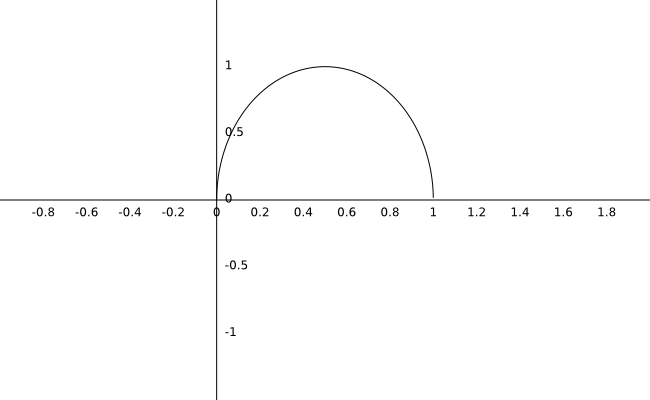
\includegraphics[width=\linewidth]{../images/x(x-1).png}
  \caption{A plot displaying $2\sqrt{(1-\epsilon_i)\epsilon_i}$}.
  \label{fig:x(x-1)}
\end{figure}

Now we have still to clarify the step $(3)$, signed as $(*)$. Indeed, this is not true for all $\mathbb{P}$.
But, if we choose:

$$
\mathbb{P}_{i+1}(t) = \frac{\mathbb{P}_{i}(t)e^{-w_i h_i(x_t) y_t}}{\E_{t\sim \mathbb{P}_i} [ e^{-w_i h_i(x_t) y_t} ]}.
$$

Then we have that $(*)$ is true. First of all we need to prove that $\sum_{t=1}^{m} \mathbb{P} = 1$.
But this is somewhat obiovous since:

\begin{align*}
\sum_{t=1}^{m} \frac{\mathbb{P}_{i}(t)e^{-w_i h_i(x_t) y_t}}{\E_{t\sim \mathbb{P}_i} [ e^{-w_i h_i(x_t) y_t} ]} = 
\sum_{t=1}^{m} \frac{\mathbb{P}_{i}(t)e^{-w_i h_i(x_t) y_t}}{\sum_{t=1}^{m} \mathbb{P}_i(t) e^{-w_i h_i(x_t) y_t} } = 
1.
\end{align*}

And note that:
$$
\mathbb{P}_{i+1}(t) = \frac{\mathbb{P}_{i}(t)e^{-w_i h_i(x_t) y_t}}{\E_{t\sim \mathbb{P}_i} [ e^{-w_i h_i(x_t) y_t} ]}.
\implies e^{-w_i h_i(x_t) y_t} = \E_{t\sim \mathbb{P}_i} [ e^{-w_i h_i(x_t) y_t} ] \frac{\mathbb{P}_{i+1}(t)}{\mathbb{P}_{i}(t)}
$$

So, we have:

\begin{align*}
\E_{t\sim \mathbb{P}_1} [\prod_{i=1}^{T} e^{-w_i h_i(x_t) y_t}] = 
\E_{t\sim \mathbb{P}_1} [\prod_{i=1}^{T} \E_{t\sim \mathbb{P}_i} [ e^{-w_i h_i(x_t) y_t} ] \frac{\mathbb{P}_{i+1}(t)}{\mathbb{P}_{i}(t)}] = \\
\sum_{t=1}^{m} \mathbb{P}_1(t) (\underbrace{\prod_{i=1}^{T} \frac{\mathbb{P}_{i+1}(t)}{\mathbb{P}_{i}(t)}}_{telescopic product} \prod_{i=1}^{T} \E_{t\sim \mathbb{P}_i} [ e^{-w_i h_i(x_t) y_t} ]) = 
\sum_{t=1}^{m} \mathbb{P}_1(t) (\frac{\mathbb{P}_{T+1}(t)}{\mathbb{P}_{1}(t)} \prod_{i=1}^{T} \E_{t\sim \mathbb{P}_i} [ e^{-w_i h_i(x_t) y_t} ]) = \\ = 
\sum_{t=1}^{m}  (\mathbb{P}_{T+1}(t) \prod_{i=1}^{T} \E_{t\sim \mathbb{P}_i} [ e^{-w_i h_i(x_t) y_t} ]) = 
\sum_{t=1}^{m}  (\mathbb{P}_{T+1}(t) \prod_{i=1}^{T} \E_{t\sim \mathbb{P}_i} [ e^{-w_i h_i(x_t) y_t} ]) = 
\prod_{i=1}^{T} \E_{t\sim \mathbb{P}_i} [ e^{-w_i h_i(x_t) y_t} ]).
\end{align*}

Now note the followings:
\begin{itemize}
	\item Adaboost Can use good predictors as a bad one, in fact, bad predictors will have high $\epsilon_i$, and so,
	a negative weight.
	\item If the i-th predictor has $\frac{1}{2}$ accuracy over samples weighted with $\mathbb{P}_i$ then it has
	no use in the classification, since it gets a weight of $0$.
\end{itemize}

\subsection{Tree stump}
Tree predictors are classifiers particularly suited for problems with discrete or non-euclidean domains, like:

$$\mathcal{X}=\{\underbrace{\{young, adult, old\}}_{age}\times\underbrace{\{yes, no\}}_{smoker}\times\underbrace{\{underweight,normal,overweight,obese\}}_{weight}\}.$$

The general idea is to take tests, functions of the form $f:\mathcal{X}\rightarrow\mathcal{Y}$ combining them in a tree
where each leaf is labeled with a class $y \in \mathcal{Y}$ and each node is a test.
Each sample $x \in \mathcal{X}$ is then routed towards a leaf and classified with the respective label.
The training set is used for two reasons: 

\begin{enumerate}
	\item $S$ is used to decide which label to assign to each leaf. Given the leaf $l$ the 
	the label $y$ assigned to $l$ is the majority of labels of samples $(x_t,y_t)\in S$ routed to $l$.
	$$l_y = majority\{y_t | (x_t,y_t) \in S \wedge x_t \text{ routed to } l\}$$
	\item $S$ can also be used in the splitting decision (adding a new test to the tree). For example, we could split
	the leaf with lower accuracy and we could add the test which maximizes the mean of the accuracies of the new leaves
	(the accuracy is measured in respect to $S$).
\end{enumerate}

Given any tree, its training error is always less than $\frac{1}{2}$ (in binary classification), 
since we apply the majority label to the leaf's class.
And, any new split can only reduce the training error.\\

Tree stumps are tree predictors with only one node, in fact, they are just tests.

\subsection{Adaboost with stumps}
Let us suppose that $\mathcal{Y} = \{-1,+1\}$, so that, we are in a binary classification setting.
The algorithm works as follow:

\begin{lstlisting}[language=Java]
Let S be the training set.
Let T be the number of boosting rounds.
Let F be set of possible tests (stumps).
Let P_1 be the uniform probability distribution over S.
For i = 1,2,...,T:
	choose a test f_i in F.
	compute the e_i training error weighted with P_i, for f_i.
	compute the predictor's weight w_i.
	compute the new probability distribution P_i+1.
Return ((w_1,..,w_T),(f_1,...,f_T)).
\end{lstlisting}

Now the only part that is unclear is about how to choose the next test.
In fact, this is not important, Adaboost works even with randomly chosen tests. But, this affects the number of iteration
required to convergence.

So, i tried the following strategies for the stump generation:
\begin{enumerate}
	\item Fully random. the next test is chosen from a pre-generated set of possible tests.
	\item A variable is chosen randomly and the best test is searched from all tests related to that variable.
	For the sake of speed if a test has an error that differs of $0.001$ from $\frac{1}{2}$ is directly chosen.
	\item The set of possible tests is shuffled and then the best is searched sequentially. Again, for the sake
    of speed if the test error differs from $\frac{1}{2}$ for more than $0.001$ then is directly chosen.
\end{enumerate}

\subsection{Cross-Validation}
Cross-validation, given a learning algorithm $A$ is a good method to approximate as closely as possible the statistical error. The idea is to run $A$ more times over different
training set and test set. The mean of different test errors should be close to the statistical error.

More precisely, given the dataset $S$. split $S$ in $k$ partitions $S_1, S_2, \dots S_k$ where each of them 
has size of $\frac{|S|}{k}$ and return:

$$\frac{1}{K}\sum_{i=1}^{i=k} l_{S_i}(A(S\setminus S_i)).$$

Often learning algorithms may have hyperparameters, so we need to test essentially different algorithms $A_1,\dots,A_r$.
We may use cross-validation to find the one with the smallest meaned test error. However,
it is possible that we have found one $A_l$ that is good on the dataset but not on the real statistical data,
in this case, we are overfitting in respect to the hyperparameters and our test error doesn't mean too much. 
So to protect ourselves from this rather unfortunate case we split $S$ in two $S_1$ and $S_2$.
$S_1$ will be used normally with the cross-validation, meanwhile, the purpose of $S_2$ is to have
unseen data to test our best algorithm.

\section{Forest Cover dataset}

The dataset is composed of $15120$ records. Each record has $56$ attributes where the first one
is a unique identifier and the last one the class (or cover type), which ranges from $1$ to $7$.
Of course, these two attributes will be excluded from the classification.
Our input data are both binary and integers and we have variables as Elevation, Aspect, Slope, etc.
Lastly, all classes are the $\sim 14\%$ of the whole dataset, so, there are not over represented classes.

\section{Experiment description}
\subsection{Tests generation (stumps)}
So we have $54$ attributes: $\mathcal{X} = \mathcal{X}_1, \dots,\mathcal{X}_{54}$ and $\mathcal{Y} = \{-1,1\}$, where
each class is considered in a setting one vs all, so that, we can use binary predictors.
Each base predictor is from $ \mathcal{F} \subset \{\{1,\dots,54\}\times \mathbb{N}: \rightarrow \{True,False\}\}$.
For example, the test $f_{(14,42)}(x)$ would check if $x_{14} \leq 42$.

For each attribute $\mathcal{X}_i$ , I have collected its value appearing in the training set.
For instance, for a binary attribute, I would get $\{0,1\}$. Given this set, I have
calculated the percentile, for each $0.001\%$, so that, for a list like $[1,2,3,\dots,10000]$
I take only $[0,10,20,\dots,10000]$.

In conlusion, for an attribute $\mathcal{X}_i$ with seen values $\in [1,10000]$, I generate the list of tests
$[f_{(i,0)},f_{(i,10)}, \\f_{(1i4,20)},\dots, f_{(i,10000)}]$. This choice is just for the sake of
not having too many tests.

\subsection{The test choice}
Since Adaboost benefits of strongly erroneous or accurate predictors, it makes much sense to search
for these types of predictors. So, when we want to know how a predictor behaves at the i-th step of Adaboost
we just need to compute. 
$$\epsilon_f = \mathbb{P}_i(f(x_t) y_t = -1)$$
The far the predictor strays from $\frac{1}{2}$ the better it is.
Again, the strategies adopted for the search are: fully random, shuffled best and random attribute best test.

\subsection{Measures}
I have measured three common metrics: accuracy, precision, and recall.
Each one of the previous can be computed easily by computing the followings:
\begin{itemize}
	\item true positives:
	$$tp = |\{(x,y)\in S : h(x) = 1 \wedge y = 1\}|.$$
	\item false positives:
	$$fp = |\{(x,y)\in S : h(x) = 1 \wedge y = 0\}|.$$
	\item true negatives:
	$$tp = |\{(x,y)\in S : h(x) = 0 \wedge y = 0\}|.$$
	\item false negatives:
	$$fn = |\{(x,y)\in S : h(x) = 0 \wedge y = 1\}|.$$
\end{itemize}
where:
\begin{itemize}
	\item Accuracy is the rate of correct predictions against all predictions.
	$$accuracy = \frac{tp+tn}{tp+fn+fp+tn}$$
	\item Recall is the rate of true labels classified as true over all true labels.
	$$recall = \frac{tp}{tp+fn}$$
	\item Precision is the rate of true labels classified as true against all true predictions.
	$$recall = \frac{tp}{tp+fn}$$

\end{itemize}

\subsection{Bringing it all together}
How does all works:
\begin{enumerate}
	\item Get the list of all records $S$.
	\item Generate from $S$ the possible tests $\mathcal{F}$.
	\item Split the dataset in two $S_1$ and $S_2$, such that, $|S_1| = \frac{1}{3}|S_2|$.
	\item Choose a strategy from $\{\text{random},\text{shuffled best},\text{random attribute best test}\}$.
	\item Choose a class $c \in \{1,2,3,4,5,6,7\}$.
	\item Generate the one-vs-all version of $S_1$, call it $S_{vs}$. 
	$$S_{vs} = \{(x,0)|(x,c') \in S \land c' \neq c\} \cup \{(x,1)|(x,c) \in S\}.$$
	\item Now partition $S_{vs}$ in $S_{vs_1}, S_{vs_2},S_{vs_3},S_{vs_4}$.
	\item Train the predictor $h_{c,strategy, S_{vs_j}}$ with Adaboost and $\mathcal{F}$ over $S_1 \setminus S_{vs_j}$.
	\item Test the prdictor $h_{c,strategy, S_{vs_j}}$ over $S_{vs_j}$.
	\item Repeat from $8.$ for all $j \in \{1,2,3,4\}$.
	\item Repeat from $5.$ for all $c \in \{1,2,3,4,5,6,7\}$.
	\item Mean all the test error obtained for ceratain strategy, call it $\epsilon_{strategy}$.
	\item Repeat from $4.$ for all $strategy \in \{\text{random},\text{shuffled best},\text{random attribute best test}\}$.
	\item find $bestStrategy = \underset{strategy}{argmin}\{\epsilon_{random},\epsilon_{shuffled best},\epsilon_{random attribute best test}\}$.
	\item Train again a predictor $h$ with adaboost, but this time over all $S_1$ with the $bestStrategy$.
	\item Compute the test error of $h$ on $S_2$.

\end{enumerate}

\section{Experiment results}

Now we will compare results obtained for different strategies and different classes.
The best strategy between the one listed is \textit{random attribute best choice} which has 
reached a meaned (from different classes) test error of $0.922$ using $1001$ stump predictors.

\newpage
lets start comparing results for the most hard class (class 2):
\begin{multicols}{2}

	\begin{minipage}[t]{1\columnwidth}
	\begin{center}
	\textbf{Random.}\par\medskip
	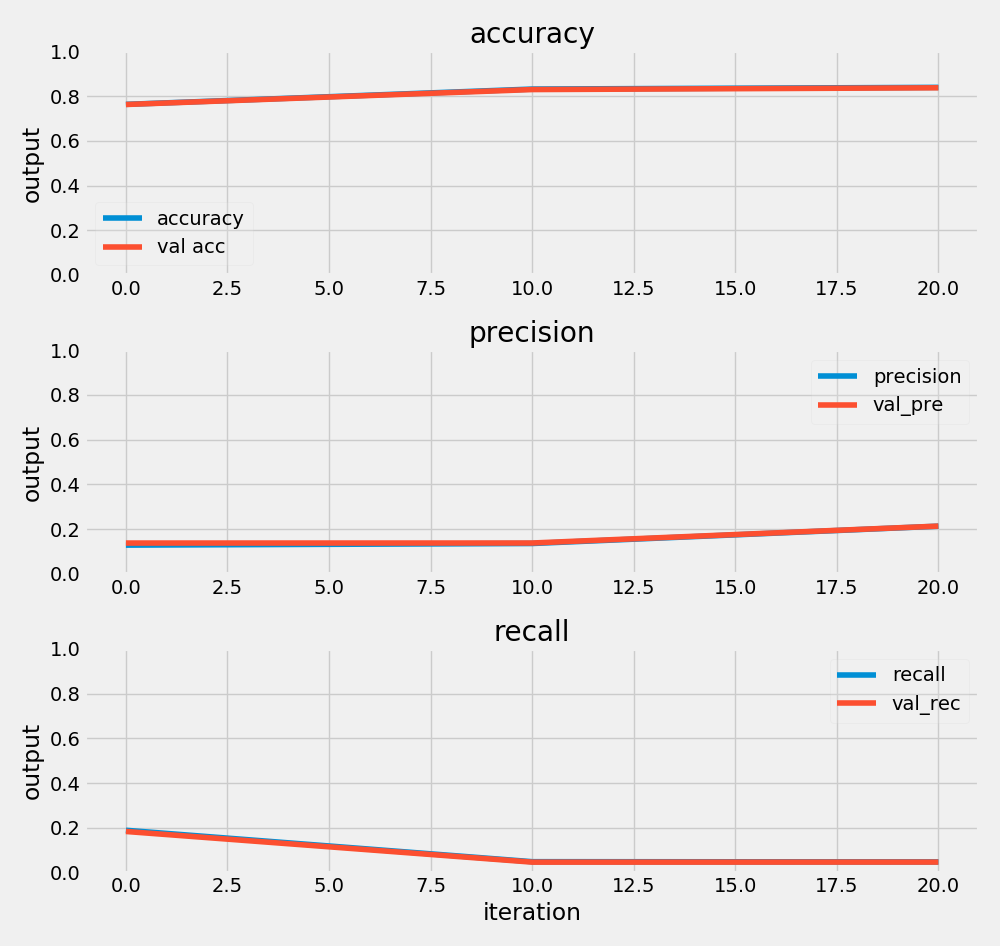
\includegraphics[width=0.9\columnwidth]{../images/random_choice_class_2_cross_val_4.png}
	\captionof{figure}{A plot displaying the results for random choice strategy for class 2 with 
	4 partitions of cross-validation.}
	\label{random}
	\end{center}
	\end{minipage}

	\begin{minipage}[t]{1\columnwidth}
	\begin{center}
	\textbf{Shuffled Best.}\par\medskip
	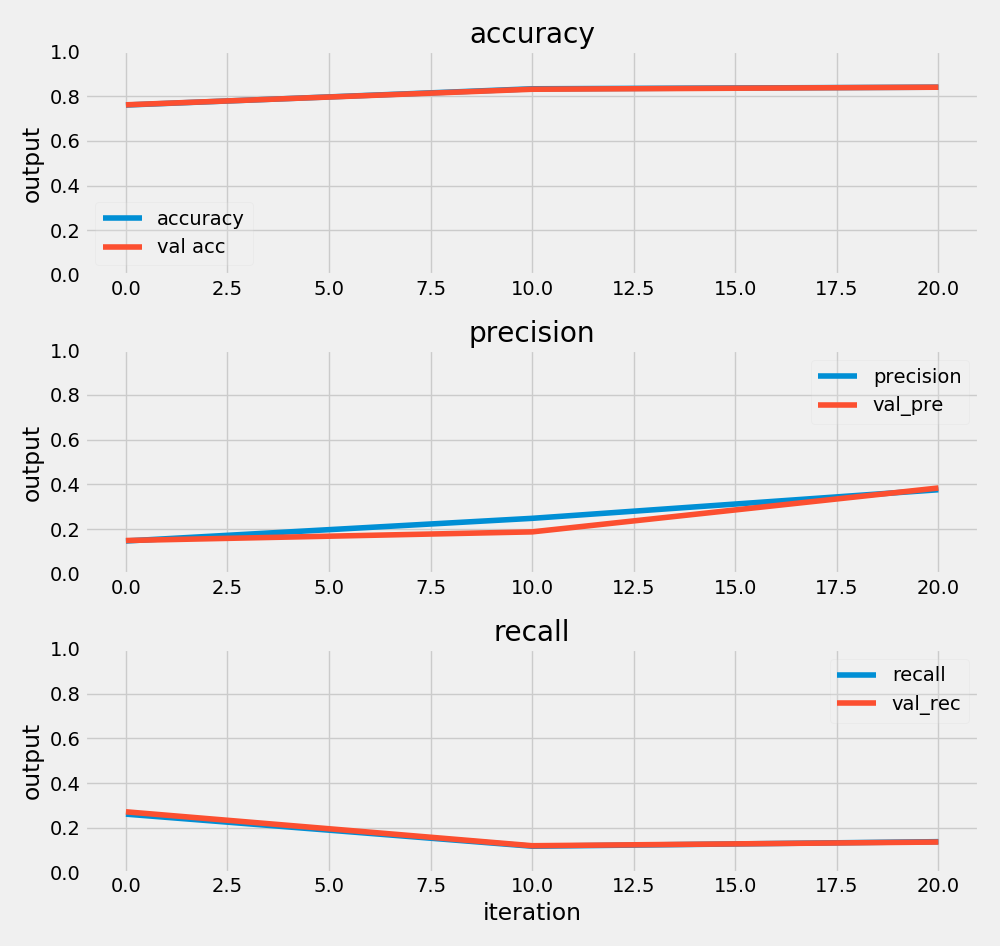
\includegraphics[width=0.9\columnwidth]{../images/best_with_threshold_class_2_cross_val_4.png}
	\captionof{figure}{A plot displaying the results for shuffled best test strategy for class 2 with 
	4 partitions of cross-validation.}
	\label{shuffled}
	\end{center}
	\end{minipage}

	\begin{minipage}[t]{1\columnwidth}
	\begin{center}
	\textbf{Random attribute best test.}\par\medskip
	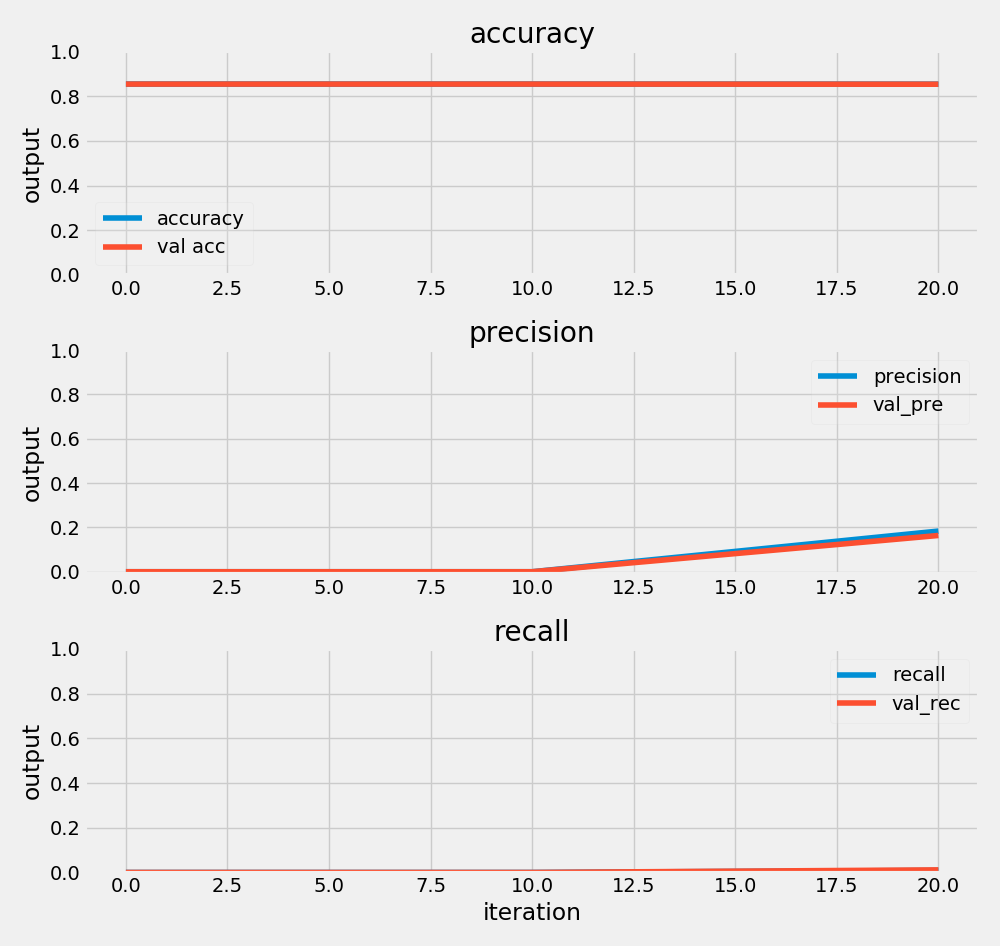
\includegraphics[width=0.9\columnwidth]{../images/random_selctor_best_test_class_2_cross_val_4.png}
	\captionof{figure}{A plot displaying the results for random attribute best test strategy for class 2 with 
	4 partitions of cross-validation.}
	\label{best}
	\end{center}
	\end{minipage}
	\text{ }
	\\*
	Here the best class accuracy barely reaches $90\%$, And recall is extremely low, which means that
	actually, we are not able to classify well the data. Instead, the $90\%$ seems even too good, and probably
	the predictor classifies most of the label as \textit{false}. This is no surprise since the large majority
	of them are \textit{false} (about $\sim 85 \%$).
	
	As we can see the \textit{random} strategy is the worst behaving one, and despite being the fastest, even after
	1000 Adaboost's iteration it doesn't catch up with the others. Meanwhile \textit{Random attribute best test} seems to
	converge faster, in number of iteration, than others.\\
\end{multicols}
\newpage

Now lets see for the most easy class (class4):
\begin{multicols}{2}

	\begin{minipage}[t]{1\columnwidth}
	\begin{center}
	\textbf{Random.}\par\medskip
	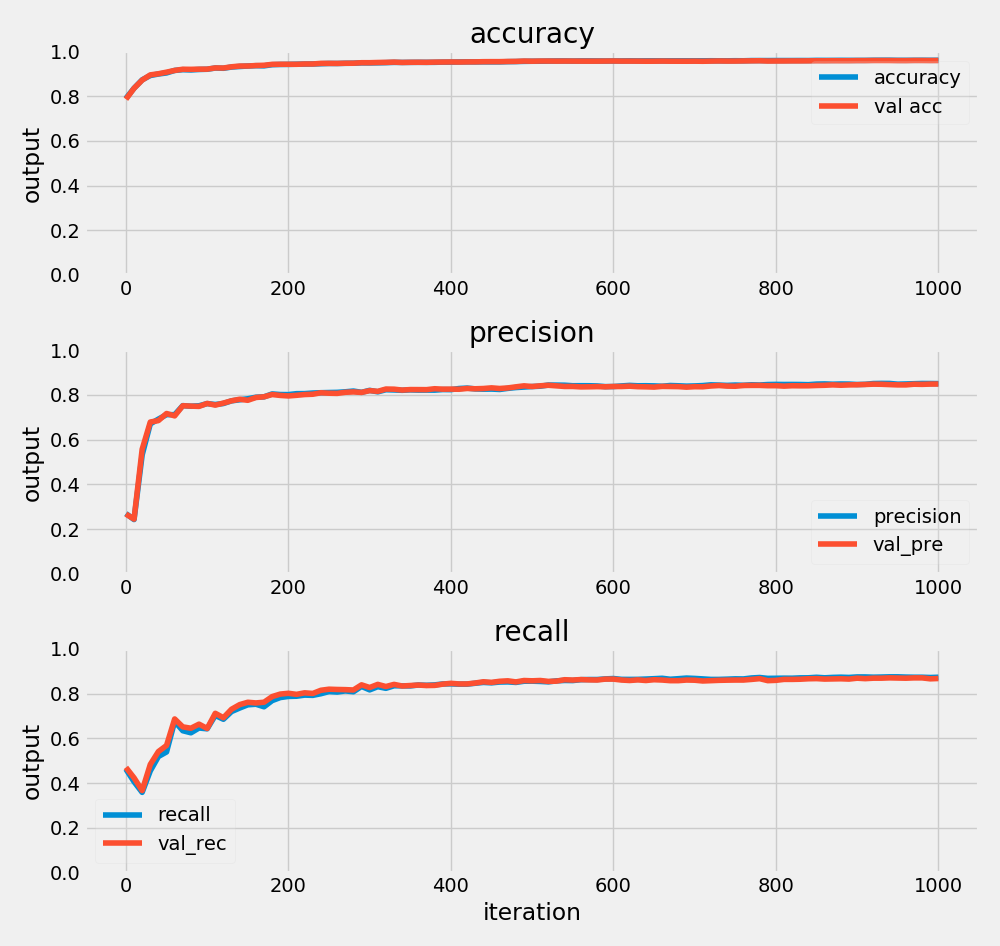
\includegraphics[width=0.9\columnwidth]{../images/random_choice_class_4_cross_val_4.png}
	\captionof{figure}{A plot displaying the results for random choice strategy for class 4 with 
	4 partitions of cross-validation.}
	\label{random}
	\end{center}
	\end{minipage}

	\begin{minipage}[t]{1\columnwidth}
	\begin{center}
	\textbf{Shuffled Best.}\par\medskip
	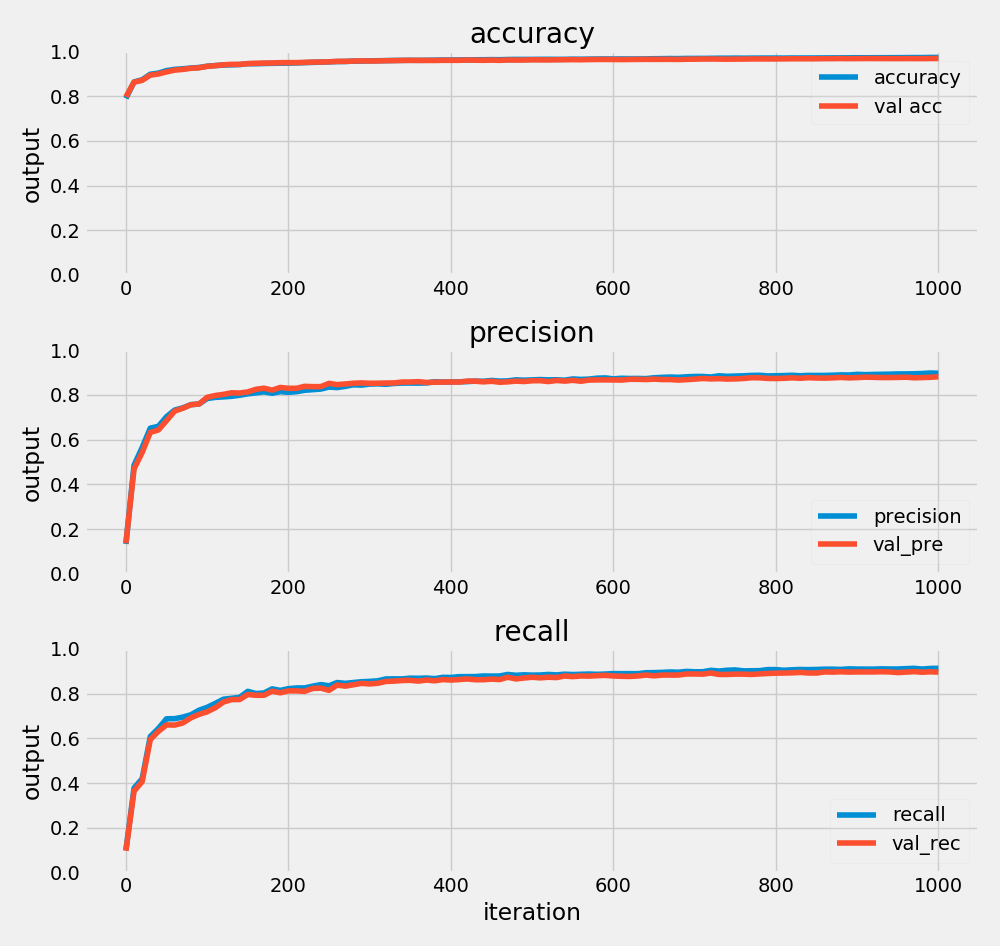
\includegraphics[width=0.9\columnwidth]{../images/best_with_threshold_class_4_cross_val_4.png}
	\captionof{figure}{A plot displaying the results for shuffled best test strategy for class 4 with 
	4 partitions of cross-validation.}
	\label{shuffled}
	\end{center}
	\end{minipage}

	\begin{minipage}[t]{1\columnwidth}
	\begin{center}
	\textbf{Random attribute best test.}\par\medskip
	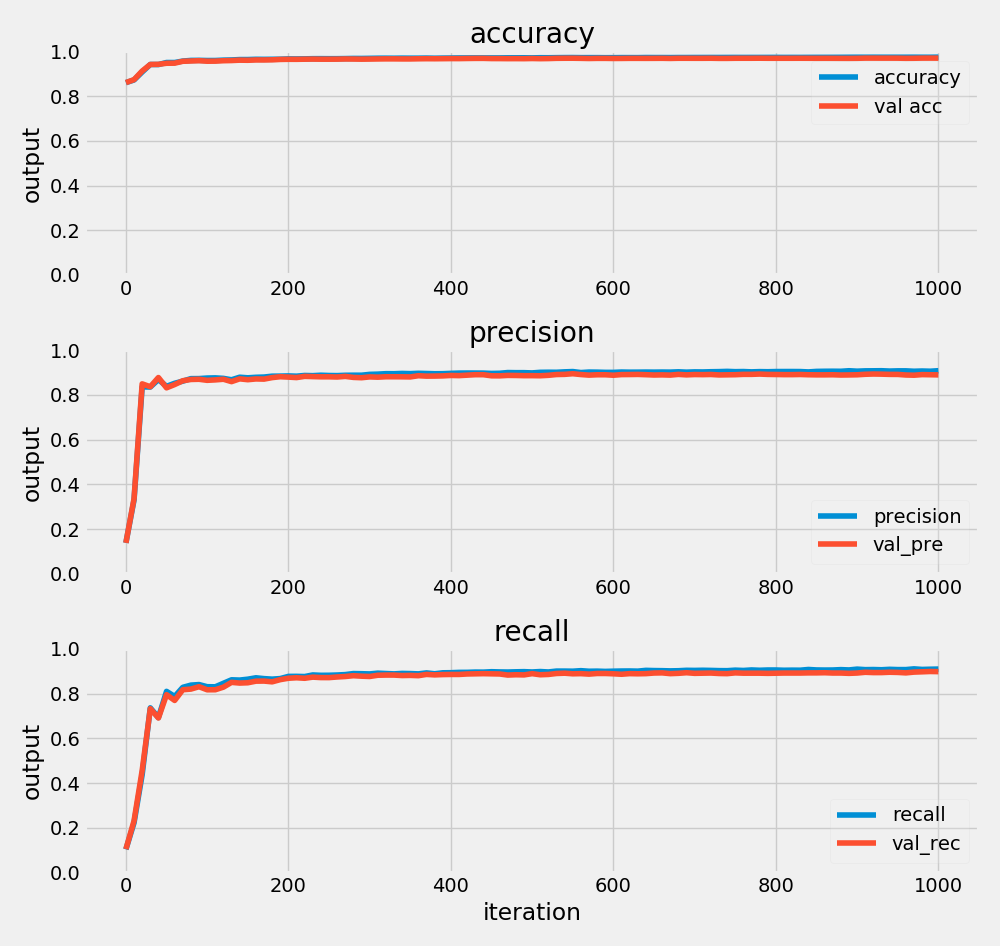
\includegraphics[width=0.9\columnwidth]{../images/random_selctor_best_test_class_4_cross_val_4.png}
	\captionof{figure}{A plot displaying the results for random attribute best test strategy for class 4 with 
	4 partitions of cross-validation.}
	\label{best}
	\end{center}
	\end{minipage}
	\text{ }
	\\*
	Here, the previous problem doesn't seem to appear. 
	Even if the majority of labels is false, the predictor has learned well how to distinguish class 4 from the other.
	
	The previous reasoning applies also in this case, and the best strategy seems to be \textit{random attribute best test}
	Here the best class accuracy reaches $\sim 97\%$. 
\end{multicols}
\newpage


Finally, we have ascertained that the strategy which reaches the best results and faster is \textit{random attribute best test}.
And now, we show the values obtained when this algorithm is trained on the whole validation data and tested on
completely unseen records:

 \begin{multicols}{2}

	\begin{minipage}[t]{1\columnwidth}
	\begin{center}
	\textbf{Class 1.}\par\medskip
	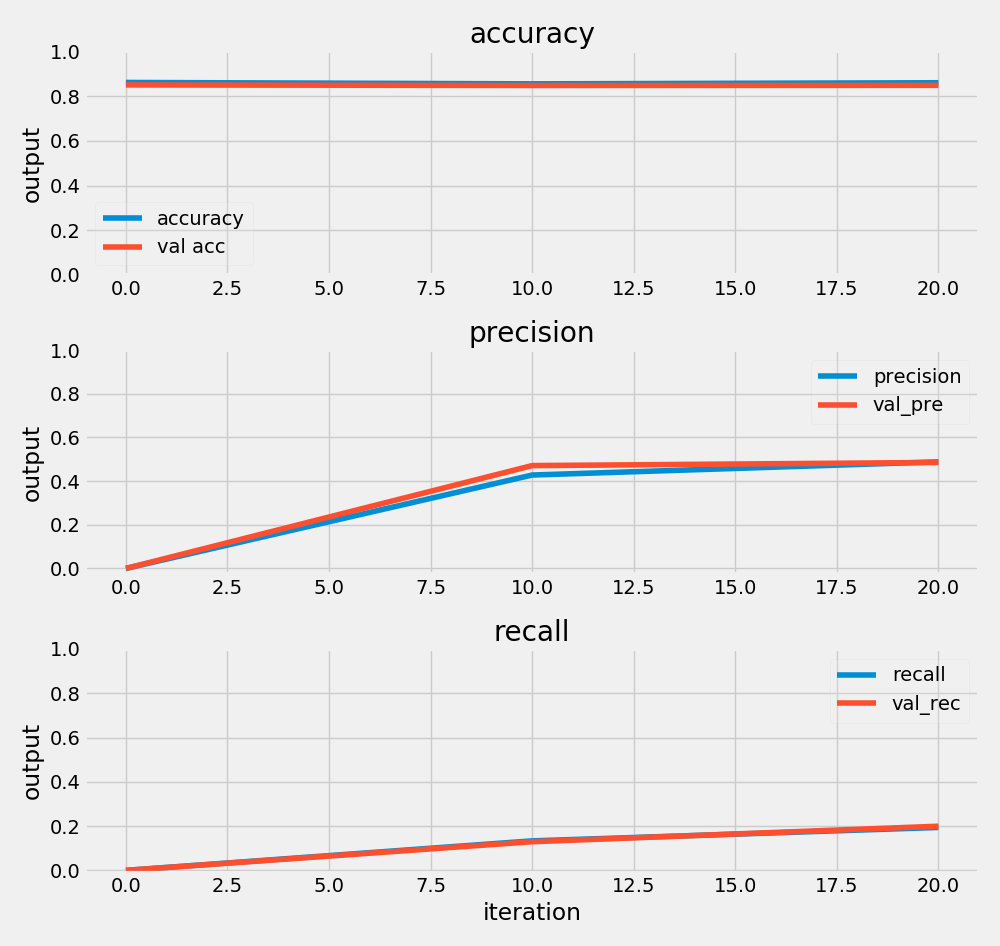
\includegraphics[width=0.9\columnwidth]{../images/best_predictor_class_1_cross_val_1.png}
	\captionof{figure}{A plot displaying the results for random attribute best test strategy for class 1 without cross-validation.}
	\label{best}
	\end{center}
	\end{minipage}

	\begin{minipage}[t]{1\columnwidth}
	\begin{center}
	\textbf{Class 2.}\par\medskip
	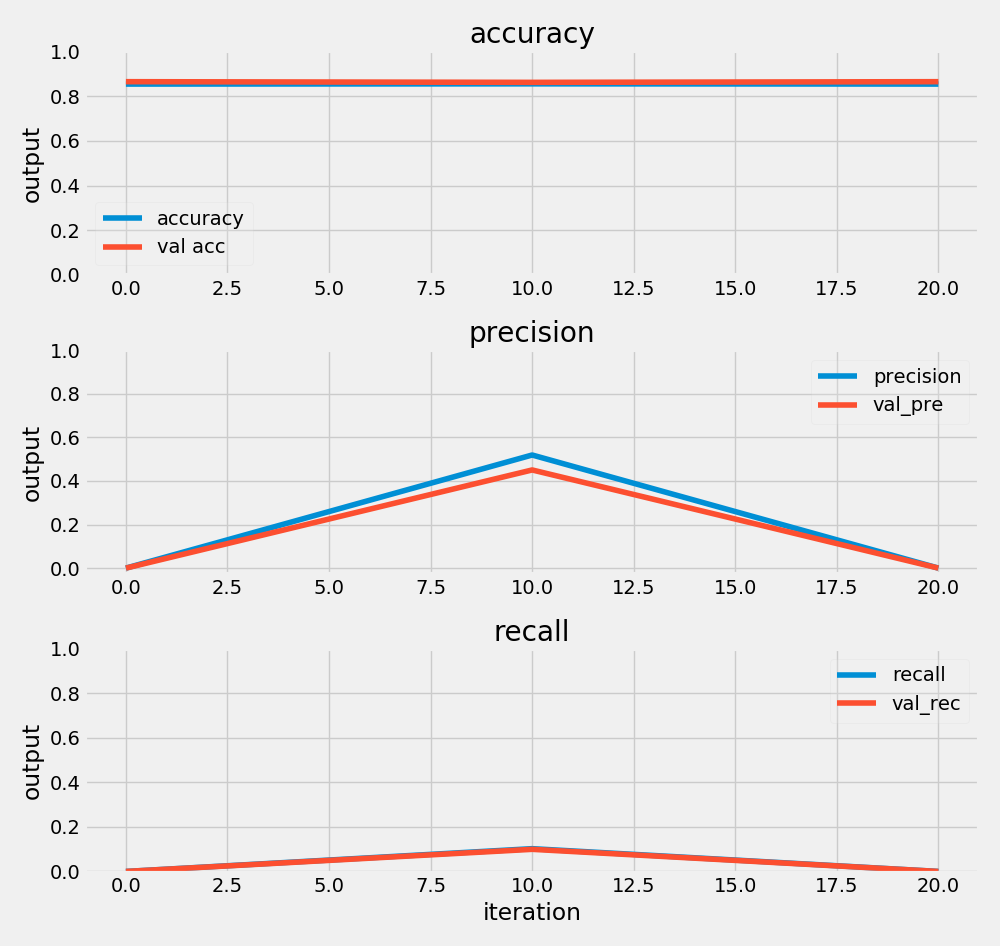
\includegraphics[width=0.9\columnwidth]{../images/best_predictor_class_2_cross_val_1.png}
	\captionof{figure}{A plot displaying the results for random attribute best test strategy for class 2 without cross-validation.}
	\label{best}
	\end{center}
	\end{minipage}


	\begin{minipage}[t]{1\columnwidth}
	\begin{center}
	\textbf{Class 3.}\par\medskip
	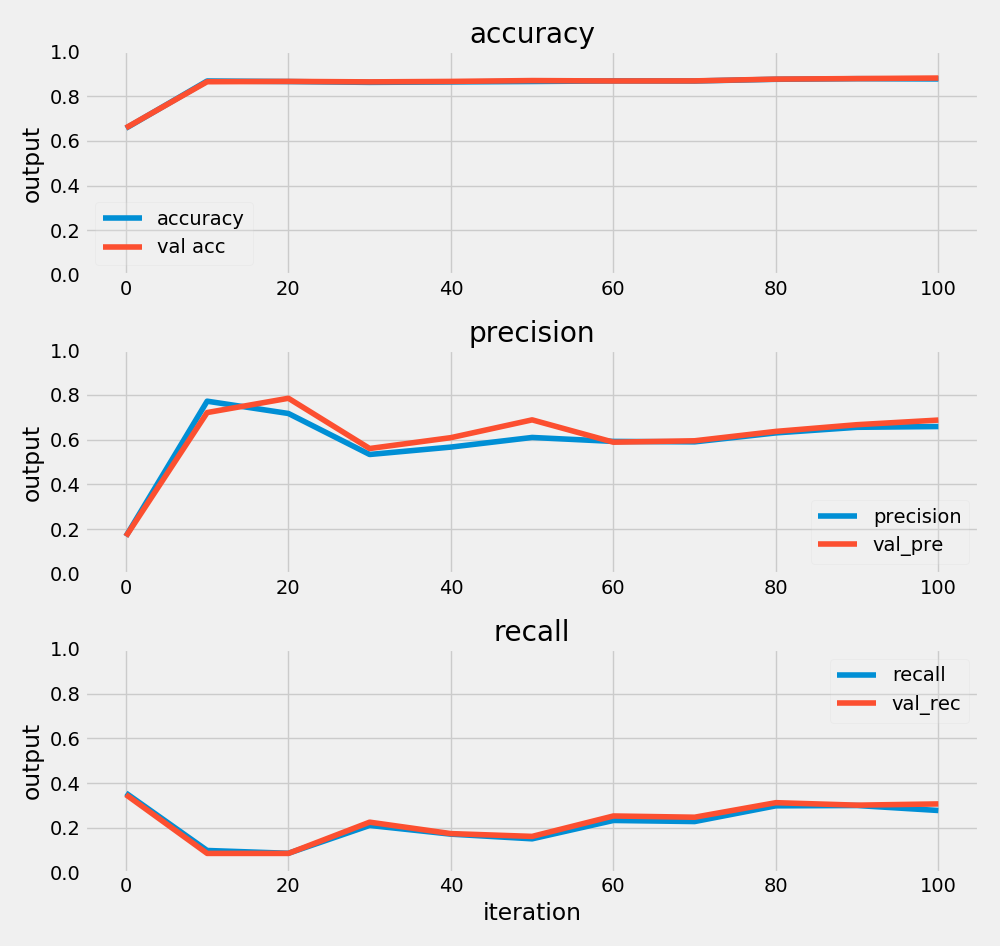
\includegraphics[width=0.9\columnwidth]{../images/best_predictor_class_3_cross_val_1.png}
	\captionof{figure}{A plot displaying the results for random attribute best test strategy for class 3 without cross-validation.}
	\label{best}
	\end{center}
	\end{minipage}

	\begin{minipage}[t]{1\columnwidth}
	\begin{center}
	\textbf{Class 4.}\par\medskip
	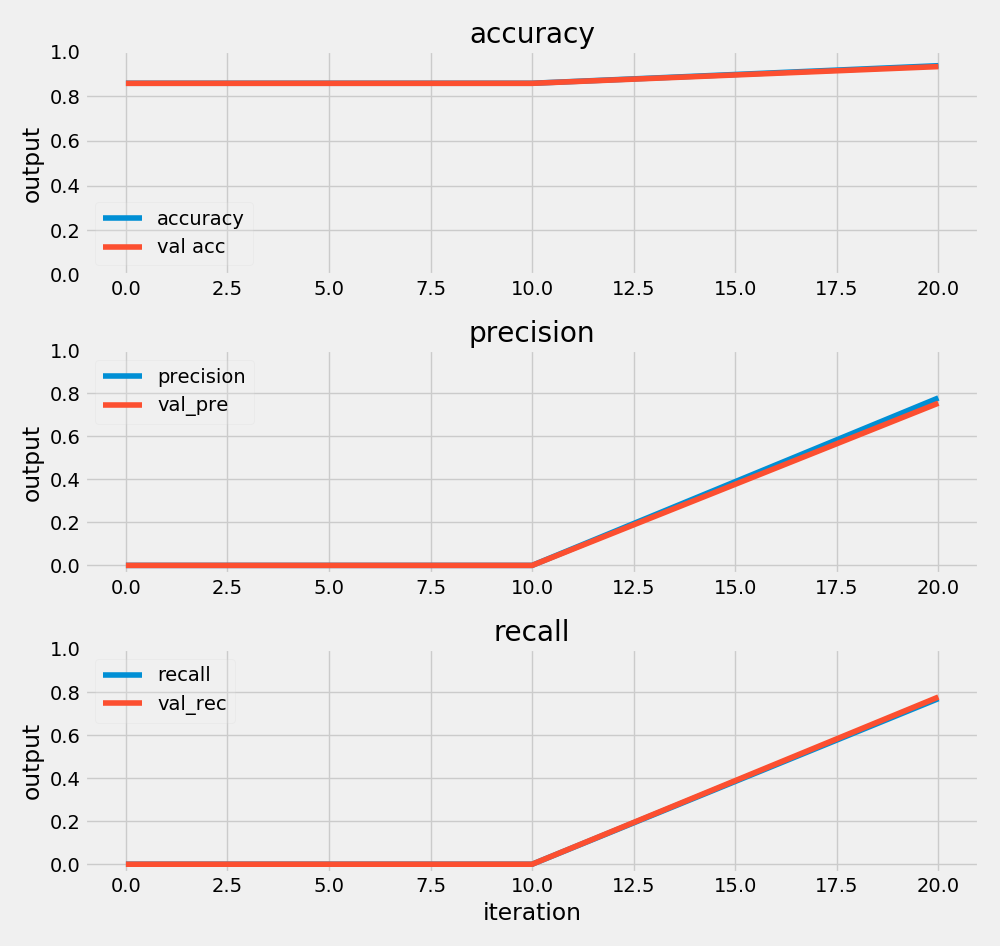
\includegraphics[width=0.9\columnwidth]{../images/best_predictor_class_4_cross_val_1.png}
	\captionof{figure}{A plot displaying the results for random attribute best test strategy for class 4 without cross-validation.}
	\label{best}
	\end{center}
	\end{minipage}

	\begin{minipage}[t]{1\columnwidth}
	\begin{center}
	\textbf{Class 5.}\par\medskip
	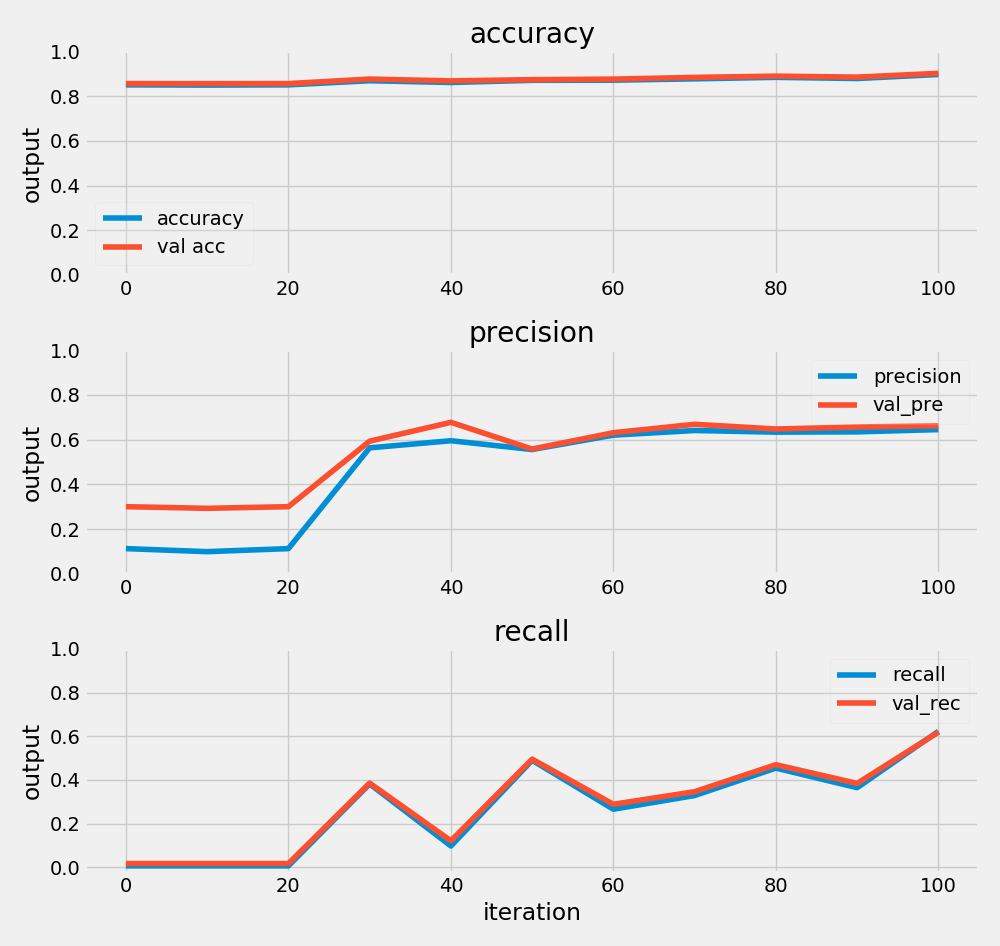
\includegraphics[width=0.9\columnwidth]{../images/best_predictor_class_5_cross_val_1.png}
	\captionof{figure}{A plot displaying the results for random attribute best test strategy for class 5 without cross-validation.}
	\label{best}
	\end{center}
	\end{minipage}

	\begin{minipage}[t]{1\columnwidth}
	\begin{center}
	\textbf{Class 6.}\par\medskip
	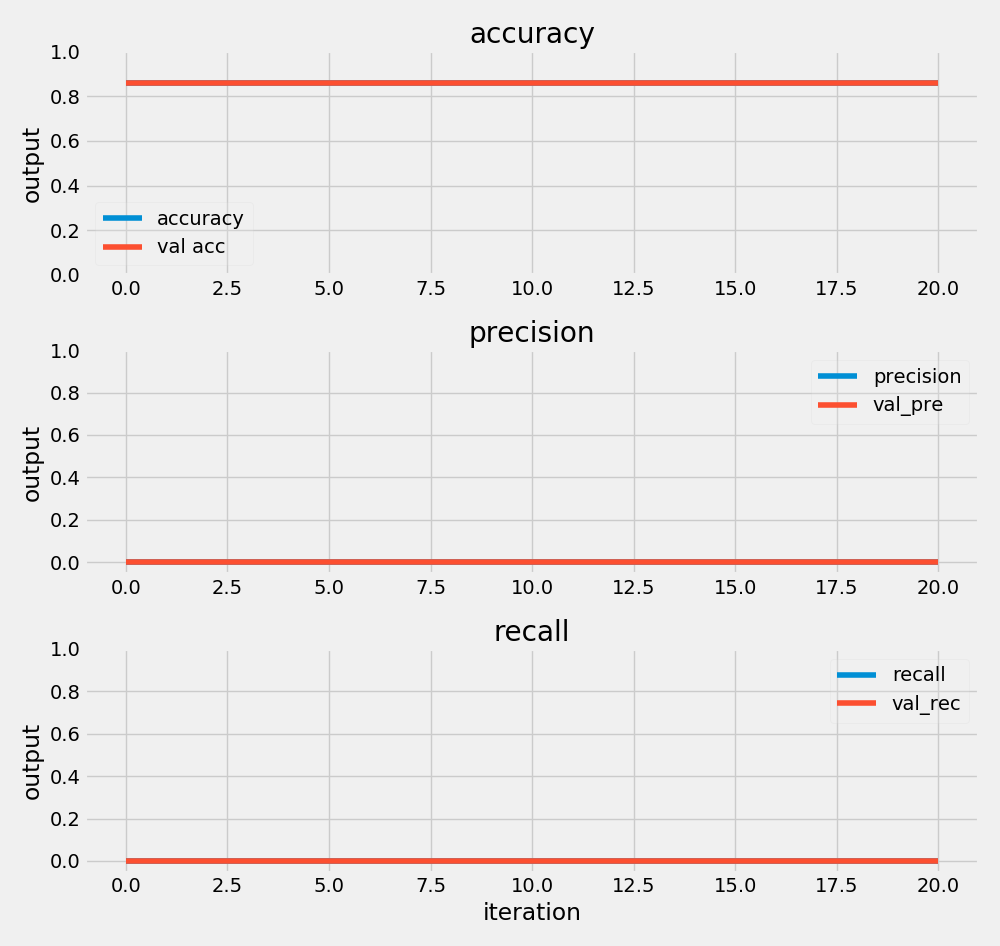
\includegraphics[width=0.9\columnwidth]{../images/best_predictor_class_6_cross_val_1.png}
	\captionof{figure}{A plot displaying the results for random attribute best test strategy for class 6 without cross-validation.}
	\label{best}
	\end{center}
	\end{minipage}

	\begin{minipage}[t]{1\columnwidth}
	\begin{center}
	\textbf{Class 7.}\par\medskip
	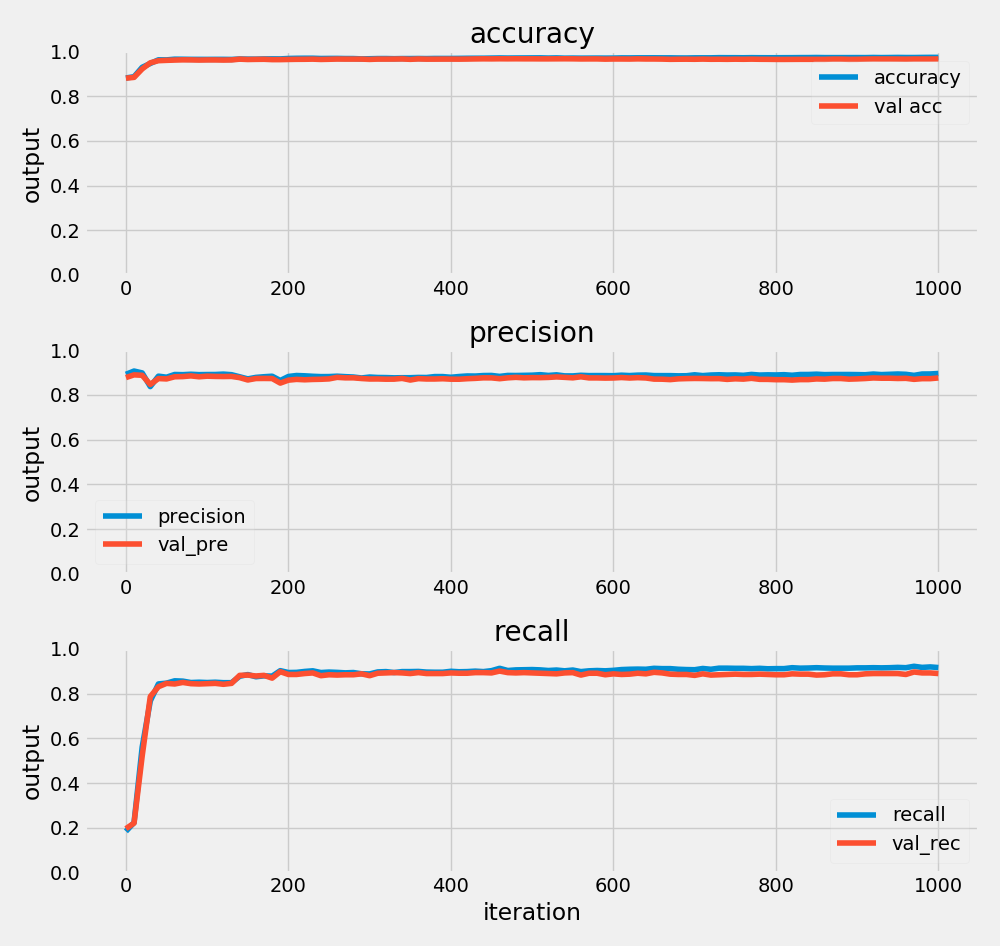
\includegraphics[width=0.9\columnwidth]{../images/best_predictor_class_7_cross_val_1.png}
	\captionof{figure}{A plot displaying the results for random attribute best test strategy for class 7 without cross-validation.}
	\label{best}
	\end{center}
	\end{minipage}
	\text{ }
	\\*
	In conclusion, even with more training data classes $1,2,3$ and $6$ seems a bit problematic, 
	meanwhile, classes $4,5$ and $7$ behave very well. 

\end{multicols}


\end{document}

